% Chương 2
\chapter{TỔNG QUAN} % Tên của chương

\label{Chapter2} % Để trích dẫn chương này ở chỗ nào đó trong bài, hãy sử dụng lệnh \ref{Chapter1} 

%----------------------------------------------------------------------------------------

% Định nghĩa một số lệnh cần thiết để điều chỉnh định dạng cho một số nội dung nhất định trong bài
\renewcommand{\keyword}[1]{\textbf{#1}}
\renewcommand{\tabhead}[1]{\textbf{#1}}
\renewcommand{\code}[1]{\texttt{#1}}
\renewcommand{\file}[1]{\texttt{\bfseries#1}}
\renewcommand{\option}[1]{\texttt{\itshape#1}}
\setcounter{secnumdepth}{3} 
%----------------------------------------------------------------------------------------

\section{Tổng quan về bài toán nhận diện chữ viết tay}


Nhận diện chữ viết tay (Handwritten Text Recognition - HTR) là một bài toán quan trọng trong lĩnh vực xử lý ảnh và thị giác máy tính, với mục tiêu chuyển đổi nội dung chữ viết tay từ ảnh sang dạng văn bản có thể xử lý được bằng máy tính \cite{Reference5, Reference8}. Bài toán này đóng vai trò quan trọng trong việc số hóa tài liệu, tự động hóa quy trình nhập liệu và lưu trữ thông tin.

HTR được chia thành hai loại chính: nhận diện chữ viết tay trực tuyến (online) và ngoại tuyến (offline). Trong đó, bài toán offline HTR chỉ sử dụng ảnh tĩnh của chữ viết tay, không có thông tin về quá trình viết, do đó khó hơn và phổ biến hơn trong thực tế \cite{Reference8}.

Ngoài ra, bài toán HTR có thể được chia theo mức độ xử lý, bao gồm nhận diện ở mức ký tự (character-level), từ (word-level) và dòng (line-level). Trong đề tài này, bài toán được tập trung ở mức dòng chữ (line-level), trong đó mỗi ảnh đầu vào tương ứng với một chuỗi ký tự cần được nhận diện.

\section{Các thách thức trong nhận diện chữ viết tay tiếng việt}

Mặc dù lĩnh vực nhận diện chữ viết tay tiếng việt đã đạt được nhiều tiến bộ nhờ sự phát triển của các phương pháp học sâu, đây vẫn là một bài toán thách thức do tính không chuẩn hóa và biến thiên cao của dữ liệu đầu vào.

\subsection{Một số thách thức của tiếng Việt}

Trước hết, sự đa dạng trong phong cách chữ viết khiến các ký tự cùng một lớp có thể khác nhau đáng kể về hình dạng, độ nghiêng, độ đậm nhạt và cách thể hiện nét, gây khó khăn cho việc học đặc trưng chung của mô hình. Bên cạnh đó, hiện tượng các ký tự dính liền hoặc chồng lấn trong chữ viết tay tự nhiên làm cho việc phân đoạn trở nên phức tạp, đặc biệt đối với các phương pháp truyền thống \cite{Reference10,Reference11}.

Ngoài ra, chất lượng dữ liệu đầu vào không đồng đều, chịu ảnh hưởng bởi nhiễu, điều kiện ánh sáng và phương thức thu thập, cũng làm giảm hiệu quả nhận diện \cite{Reference9}. Các biến dạng hình học như chữ nghiêng, cong hoặc lệch dòng tiếp tục làm gia tăng độ khó của bài toán.

Đặc biệt, đối với tiếng Việt, hệ thống dấu thanh và dấu phụ phong phú làm tăng đáng kể độ phức tạp, do các dấu này thường nhỏ, dễ bị nhiễu hoặc dính với ký tự chính, từ đó ảnh hưởng đến độ chính xác của phương pháp nhận diện.

\begin{figure}[H]
    \centering
    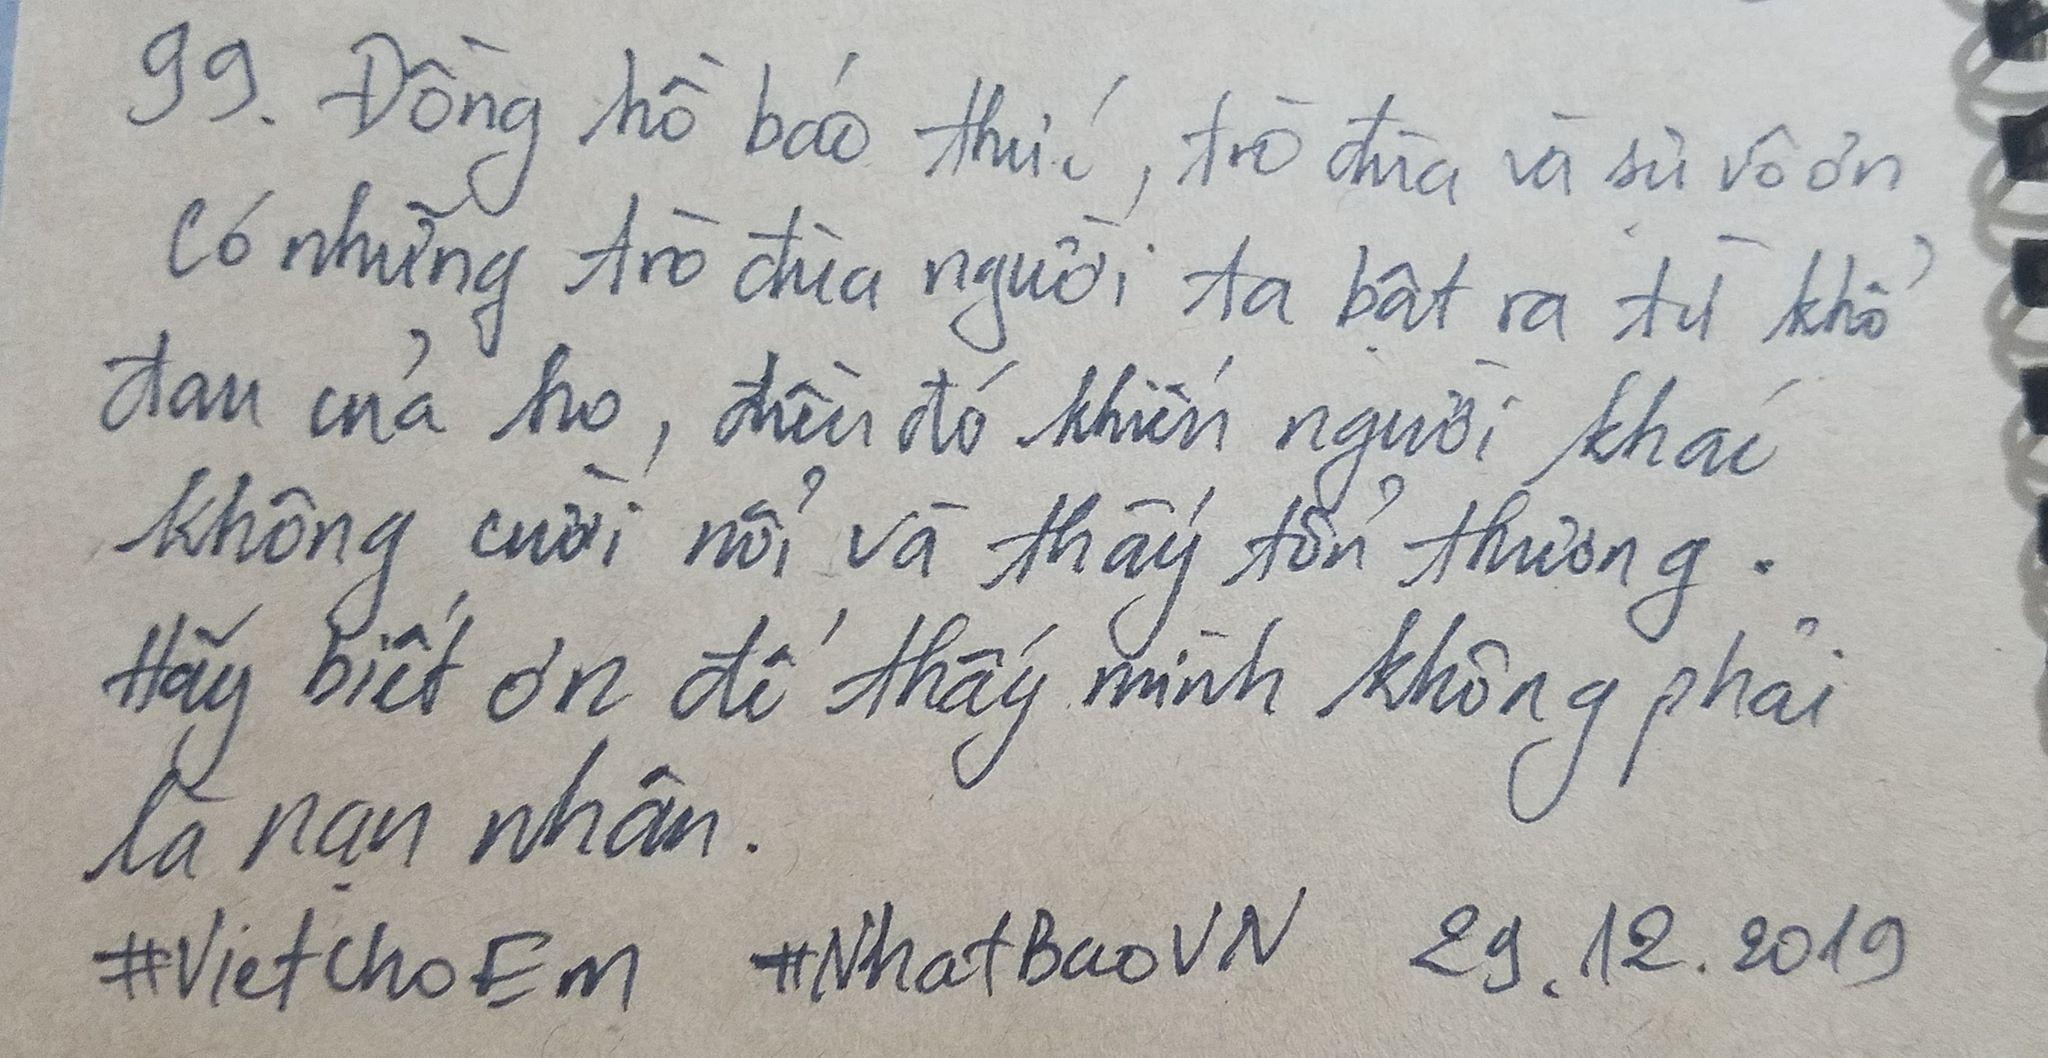
\includegraphics[width=0.7\linewidth]{Figures/Chapter2/0603.jpg}
    \caption{Hình ảnh về vấn đề của tiếng việt}
    \label{fig:handwriting_challenges}
\end{figure}

\subsection{Sự khác nhau giữ chữ đánh máy và chữ viết tay}

\begin{table}[H]
\centering
\renewcommand{\arraystretch}{1.3}
\begin{tabular}{|p{4cm}|p{5cm}|p{5cm}|}
\hline
\textbf{Tiêu chí} & \textbf{Chữ đánh máy} & \textbf{Chữ viết tay} \\
\hline
Chuẩn hóa ký tự & Cố định theo font & Phụ thuộc người viết \\
\hline
Độ đồng nhất & Gần như giống nhau & Biến thiên lớn giữa các mẫu \\
\hline
Hình dạng ký tự & Rõ ràng, ổn định & Méo, thiếu hoặc thừa nét \\
\hline
Khoảng cách ký tự & Cách đều nhau & Không đều, dễ dính chữ \\
\hline
Dòng chữ & Thẳng hàng & Có thể nghiêng, cong \\
\hline
Nhiễu dữ liệu & Thấp & Cao (mờ, rung, ánh sáng) \\
\hline
Khó khăn OCR & Dễ xử lý & Khó, dễ nhầm ký tự \\
\hline
\end{tabular}
\caption{So sánh đặc điểm giữa chữ đánh máy và chữ viết tay}
\label{tab:printed_vs_handwritten}
\end{table}

\section{Nghiên cứu liên quan}

Bài toán nhận diện chữ viết tay (Handwritten Text Recognition - HTR) đã được nghiên cứu từ lâu và trải qua nhiều giai đoạn phát triển, từ các phương pháp truyền thống dựa trên đặc trưng thủ công đến các phương pháp hiện đại dựa trên học sâu.

\subsection{Phương pháp truyền thống}

Phương pháp OCR dựa trên segmentation là hướng tiếp cận truyền thống, trong đó bài toán được chia thành nhiều bước nhỏ, đặc biệt là bước tách (phân đoạn) ký tự \cite{Reference2}. Hệ thống sẽ lần lượt thực hiện: tiền xử lý ảnh, phân đoạn dòng chữ, tách từ và cuối cùng là tách từng ký tự riêng lẻ trước khi đưa vào mô hình nhận diện.

Sau khi ký tự được tách ra, mỗi ký tự sẽ được đưa vào bộ phân loại (như SVM, k-NN hoặc mạng neural đơn giản) để nhận diện.

Ưu điểm của phương pháp này là dễ hiểu và phù hợp với văn bản in rõ ràng, có cấu trúc ổn định. Tuy nhiên, nó gặp nhiều hạn chế khi áp dụng cho chữ viết tay do hiện tượng ký tự dính liền, biến dạng hoặc không có ranh giới rõ ràng, dẫn đến sai sót trong bước phân đoạn và kéo theo giảm độ chính xác \cite{Reference2}.

\begin{figure}[H]
    \centering
    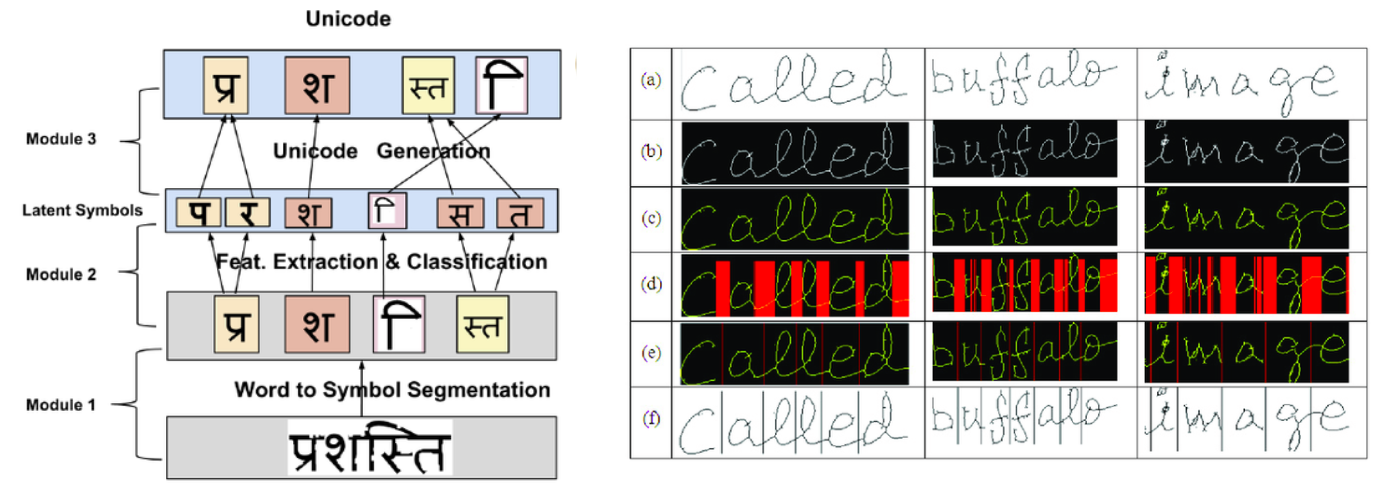
\includegraphics[width=0.9\linewidth]{Figures/Chapter2/Chapter2_1.png}
    \caption{Hình ảnh phương pháp Segmentation-based}
    \label{fig:handwriting_challenges}
\end{figure}

\subsection{Phương pháp hiện đại}

Phương pháp nhận diện chữ viết tay dựa trên Transformer là hướng tiếp cận hiện đại, trong đó bài toán được xây dựng theo mô hình end-to-end mà không cần thực hiện bước phân đoạn ký tự như các phương pháp truyền thống. Một trong những mô hình tiêu biểu là TrOCR, thường được kết hợp với mô hình thị giác mạnh như SigLIP để nâng cao khả năng trích xuất đặc trưng \cite{Reference12,Reference13}.

Hệ thống sẽ trực tiếp nhận ảnh đầu vào và thực hiện học ánh xạ từ hình ảnh sang chuỗi văn bản thông qua kiến trúc Transformer \cite{Reference14}. Cụ thể, ảnh được đưa vào encoder để trích xuất đặc trưng toàn cục, sau đó decoder sẽ sinh ra chuỗi ký tự tương ứng theo từng bước, sử dụng cơ chế attention để tập trung vào các vùng quan trọng của ảnh.

Khi kết hợp với SigLIP, mô hình có khả năng học biểu diễn hình ảnh gắn với ngữ nghĩa tốt hơn, giúp cải thiện hiệu quả trong các trường hợp chữ viết tay phức tạp, nhiễu hoặc có sự đa dạng lớn về phong cách. Ngoài ra, SigLIP còn hỗ trợ các tác vụ như phát hiện hoặc xác thực chữ ký thông qua việc so sánh embedding \cite{Reference13}.

Ưu điểm của phương pháp này là không cần tách ký tự riêng lẻ, giảm thiểu sai số do phân đoạn, đồng thời có khả năng mô hình hóa ngữ cảnh chuỗi tốt hơn nhờ cơ chế attention. Bên cạnh đó, mô hình có thể tận dụng các kỹ thuật tiền huấn luyện trên tập dữ liệu lớn để đạt hiệu năng cao.

Tuy nhiên, phương pháp này cũng tồn tại một số hạn chế như yêu cầu tài nguyên tính toán lớn, thời gian huấn luyện dài và phụ thuộc nhiều vào dữ liệu huấn luyện, ngoài ra việc triển khai và tối ưu mô hình cũng phức tạp.

\begin{figure}[H]
    \centering
    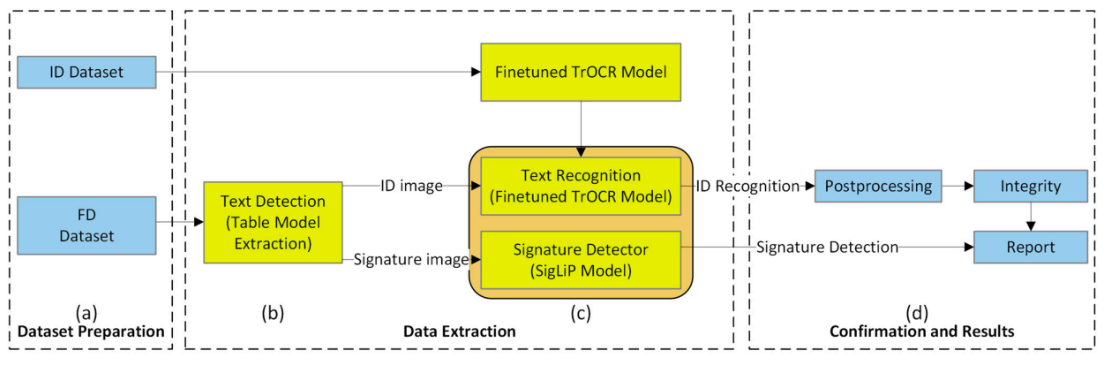
\includegraphics[width=0.9\linewidth]{Figures/Chapter2/Chapter2_2.png}
    \caption{Hình ảnh phương pháp TROCR kết hợp SigLIP}
    \label{fig:handwriting_challenges}
\end{figure}

\subsection{Phương pháp đề xuất}

Trong bối cảnh các phương pháp hiện đại như Transformer đạt hiệu năng cao nhưng đòi hỏi tài nguyên lớn và dữ liệu huấn luyện quy mô lớn, bài toán nhận diện chữ viết tay tiếng Việt vẫn cần một giải pháp cân bằng giữa hiệu quả và tính khả thi. Do đó, trong nghiên cứu này, em đề xuất sử dụng mô hình CRNN kết hợp CTC Loss như một hướng tiếp cận phù hợp và hiệu quả \cite{Reference5,Reference7}.

Phương pháp này được xây dựng theo hướng end-to-end, cho phép nhận diện trực tiếp từ ảnh đầu vào sang chuỗi ký tự đầu ra mà không cần thực hiện bước phân đoạn ký tự riêng lẻ. Cách tiếp cận này giúp đơn giản hóa quy trình xử lý và nâng cao độ chính xác tổng thể \cite{Reference5,Reference7,Reference6}.

Ảnh đầu vào trước tiên được đưa qua các lớp convolution để trích xuất đặc trưng quan trọng như nét chữ, hình dạng và cấu trúc ký tự. Sau đó, đặc trưng này được chuyển đổi thành chuỗi theo chiều ngang và đưa vào mạng BiLSTM nhằm học mối quan hệ phụ thuộc giữa các ký tự trong từ hoặc câu \cite{Reference6}. Cuối cùng, CTC Loss được sử dụng để tính toán sai số mà không cần căn chỉnh trực tiếp giữa đầu ra của mô hình và nhãn, giúp đơn giản hóa quá trình huấn luyện \cite{Reference7}.

Ưu điểm của phương pháp CRNN + CTC là kiến trúc đơn giản, dễ triển khai, không yêu cầu dữ liệu gán nhãn chi tiết theo từng ký tự và có thể huấn luyện trên các tập dữ liệu vừa và nhỏ. Ngoài ra, mô hình có tốc độ suy luận nhanh, phù hợp với các hệ thống thực tế.

Tuy nhiên, phương pháp này cũng tồn tại một số hạn chế như khả năng mô hình hóa ngữ cảnh dài hạn chưa mạnh bằng các mô hình Transformer, và hiệu năng có thể bị ảnh hưởng khi dữ liệu quá phức tạp hoặc nhiễu mạnh. Dù vậy, với sự cân bằng giữa hiệu năng và chi phí tính toán, CRNN + CTC vẫn là một lựa chọn mạnh mẽ và thực tiễn cho bài toán nhận diện chữ viết tay tiếng Việt \cite{Reference5}.

\begin{figure}[H]
    \centering
    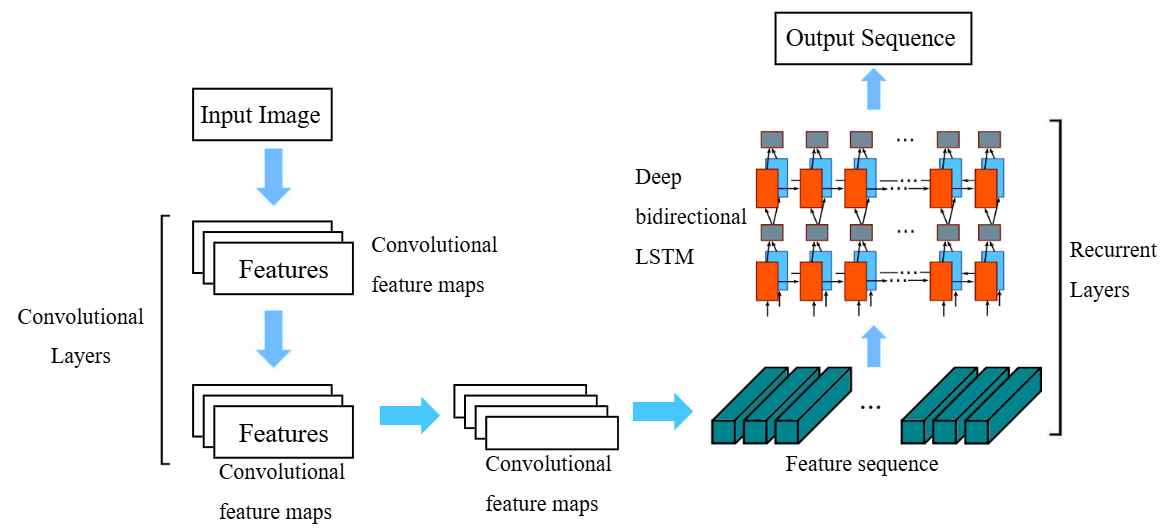
\includegraphics[width=0.9\linewidth]{Figures/Chapter2/Chapter2_3.png}
    \caption{Hình ảnh phương pháp CRNN~\cite{Reference5}}
    \label{fig:handwriting_challenges}
\end{figure}


\section{Tổng quan phương pháp}

Phương pháp nhận diện chữ viết tay tiếng Việt trong nghiên cứu này được thiết kế theo hướng tiếp cận hai giai đoạn (two-stage pipeline), bao gồm :

\begin{figure}[H]
    \centering
    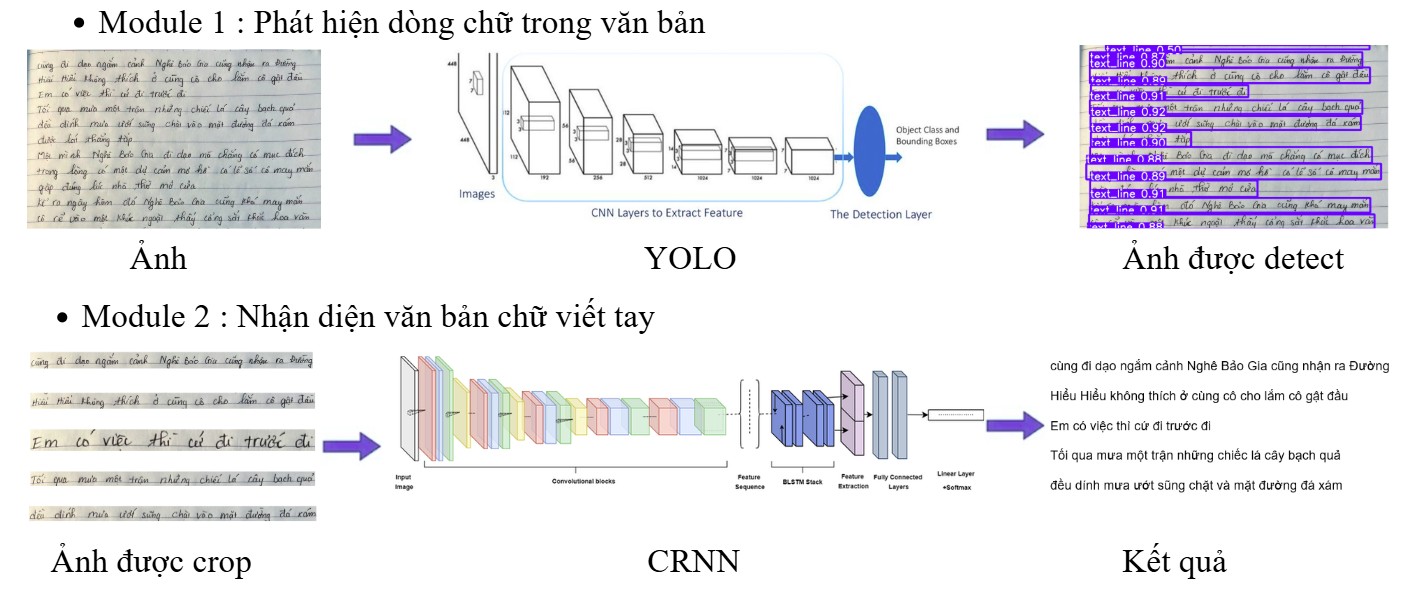
\includegraphics[width=0.9\linewidth]{Figures/Chapter3/Chapter3_1.png}
    \caption{Hình ảnh tổng quan phương pháp}
    \label{fig:handwriting_challenges}
\end{figure}

Ở giai đoạn đầu tiên, hệ thống sử dụng mô hình phát hiện đối tượng YOLO để xác định vị trí các dòng chữ trong ảnh đầu vào \cite{Reference15}. Cụ thể, ảnh tài liệu viết tay ban đầu sẽ được đưa qua mạng CNN để trích xuất đặc trưng, sau đó thông qua lớp detection để dự đoán các bounding box tương ứng với từng dòng văn bản. Kết quả của bước này là tập hợp các vùng ảnh chứa từng dòng chữ riêng biệt .

Trong giai đoạn thứ hai, mỗi dòng văn bản sau khi được cắt (crop) sẽ được đưa vào mô hình nhận diện chữ viết tay dựa trên kiến trúc CRNN (Convolutional Recurrent Neural Network) \cite{Reference5}. Mô hình này kết hợp :
\begin{itemize}
    \item Mạng CNN dùng để trích xuất đặc trưng không gian từ ảnh đầu vào \cite{Reference16}.
    \item Mạng RNN hai chiều (BiLSTM) dùng để mô hình hóa chuỗi và khai thác thông tin ngữ cảnh \cite{Reference17}.
    \item Hàm mất mát CTC dùng để thực hiện ánh xạ giữa chuỗi đặc trưng và nhãn đầu ra mà không cần căn chỉnh thủ công \cite{Reference7}.
\end{itemize}

Đầu ra cuối cùng của phương pháp là nội dung văn bản được nhận diện tương ứng với từng dòng chữ trong ảnh ban đầu.

\section{Mô hình YOLO}
\subsection{Giới thiệu}

YOLO là 1 từ viết tắt cho ‘You only look once’ (Bạn chỉ nhìn một lần) là một thuật toán phát hiện đối tượng chia hình ảnh thành một hệ thống lưới. Mỗi ô trong lưới chịu trách nhiệm phát hiện các đối tượng trong chính nó. YOLO là một trong những thuật toán phát hiện đối tượng nổi tiếng nhất do tốc độ và độ chính xác của nó \cite{Reference15}. 

YOLO là một mô hình mạng CNN cho việc phát hiện, nhận dạng, phân loại đối tượng. YOLO được tạo ra từ việc kết hợp giữa các convolutional layers và connected layers \cite{Reference15,Reference16}. Trong đó các convolutional layers sẽ trích xuất ra các feature của ảnh, còn fullconnected layers sẽ dự đoán ra xác suất đó và tọa độ của đối tượng.

\begin{figure}[H]
    \centering
    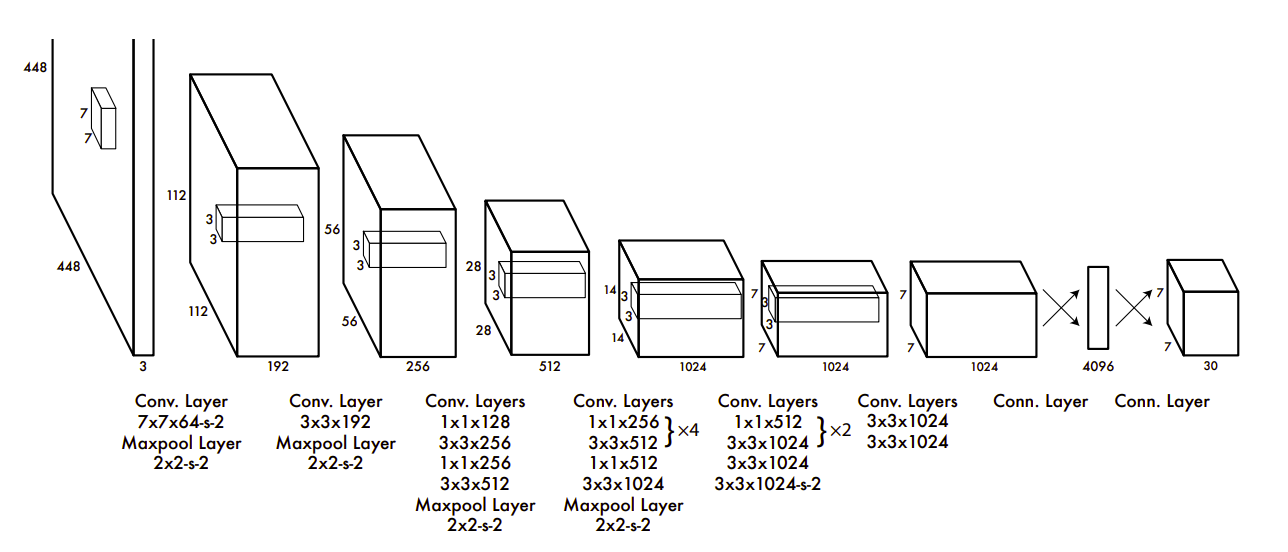
\includegraphics[width=0.9\linewidth]{Figures/Chapter3/Chapter3_2.png}
    \caption{Mô hình mạng CNN được sử dụng trong YOLO~\cite{Reference15}}
    \label{fig:handwriting_challenges}
\end{figure}

Hình ảnh đầu vào sẽ được chia thành một lưới kích thước $S \times S$, trong đó mỗi ô lưới chịu trách nhiệm phát hiện các đối tượng có tâm nằm trong ô đó. Đối với mỗi ô, mô hình sẽ dự đoán một số lượng bounding box cùng với thông tin về vị trí và xác suất lớp.

Với mỗi bounding box, mô hình dự đoán 5 tham số bao gồm $(x, y, w, h, confidence)$. Trong đó, $(x, y)$ là tọa độ tâm của bounding box tương đối so với ô lưới, còn $(w, h)$ là chiều rộng và chiều cao được chuẩn hóa theo kích thước toàn ảnh. Giá trị $confidence$ thể hiện mức độ tin cậy của bounding box, được tính dựa trên xác suất tồn tại đối tượng và độ chồng lắp giữa bounding box dự đoán và ground truth.

Ngoài ra, mỗi ô lưới còn dự đoán xác suất thuộc về các lớp đối tượng dưới dạng $Pr(Class_i \mid Object)$. Xác suất cuối cùng của một lớp được tính bằng cách kết hợp giữa xác suất lớp và $confidence$ của bounding box.

\subsection{YOLO26}

YOLO26 (hay YOLOv26) là thế hệ mới nhất thuộc họ mô hình phát hiện đối tượng You Only Look Once (YOLO) do Ultralytics phát triển, được giới thiệu vào khoảng cuối năm 2025 \cite{Reference18,Reference19}. Khác với các phiên bản trước chủ yếu tập trung vào việc gia tăng độ chính xác thông qua việc mở rộng kích thước mô hình, YOLO26 được thiết kế lại nhằm tối ưu hóa cho việc triển khai trên các thiết bị biên (edge devices), hệ thống nhúng và môi trường có tài nguyên hạn chế.

\begin{figure}[H]
    \centering
    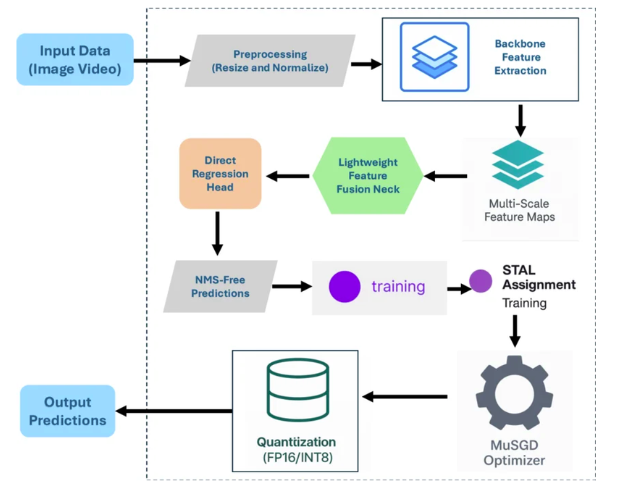
\includegraphics[height=8cm, keepaspectratio]{Figures/Chapter2/Chapter2_9.png}
    \caption{Kiến trúc tổng quan YOLO26~\cite{Reference18}}
    \label{fig:handwriting_challenges}
\end{figure}

\subsubsection*{1. Kiến trúc NMS-Free}

Các phiên bản YOLO trước đây (như YOLOv8, YOLOv9) yêu cầu bước hậu xử lý Non-Maximum Suppression (NMS) để loại bỏ các bounding box trùng lặp. Tuy nhiên, YOLO26 được thiết kế theo hướng end-to-end hoàn chỉnh, cho phép mô hình trực tiếp xuất ra các dự đoán cuối cùng mà không cần áp dụng NMS \cite{Reference18}.

Việc loại bỏ bước NMS giúp giảm độ trễ của toàn hệ thống và đơn giản hóa pipeline suy luận, đặc biệt phù hợp với các ứng dụng thời gian thực.

\begin{figure}[H]
    \centering
    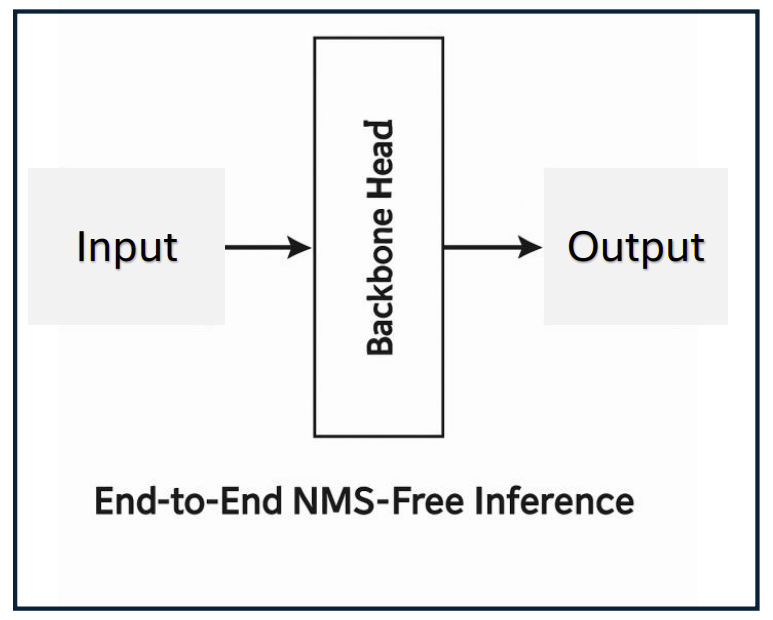
\includegraphics[height=5cm, keepaspectratio]{Figures/Chapter2/Chapter2_4.png}
    \caption{Kiến trúc NMS-Free~\cite{Reference18}}
    \label{fig:handwriting_challenges}
\end{figure}

\subsubsection*{2. Loại bỏ Distribution Focal Loss}

Trong các phiên bản trước, Distribution Focal Loss (DFL) được sử dụng để cải thiện độ chính xác của bounding box. Tuy nhiên, DFL gây khó khăn trong việc chuyển đổi mô hình sang các định dạng triển khai như TensorRT, ONNX hay CoreML.

YOLO26 loại bỏ hoàn toàn DFL, giúp quá trình export và triển khai mô hình trở nên đơn giản, ổn định và tương thích tốt hơn với phần cứng \cite{Reference18}.

\begin{figure}[H]
    \centering
    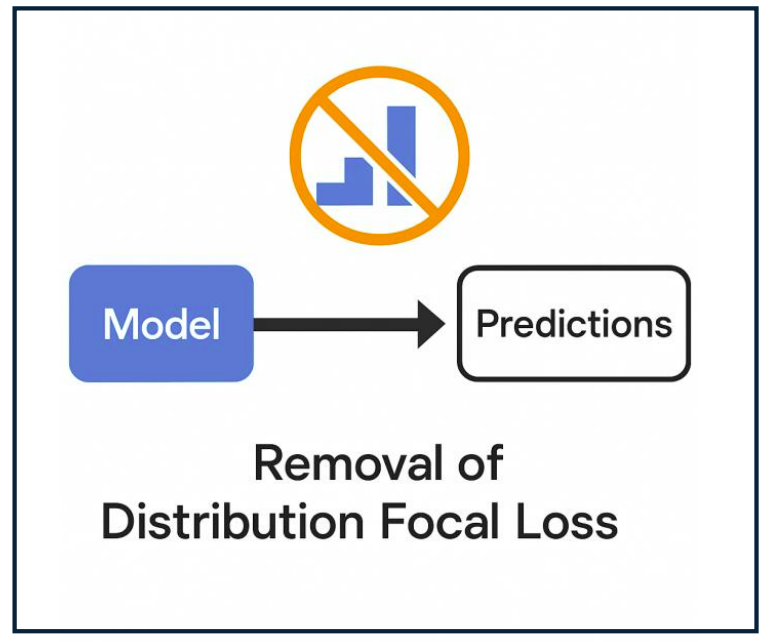
\includegraphics[height=5cm, keepaspectratio]{Figures/Chapter2/Chapter2_5.png}
    \caption{Loại bỏ DFL~\cite{Reference18}}
    \label{fig:handwriting_challenges}
\end{figure}

\subsubsection*{3. Tối ưu phát hiện vật thể nhỏ}

YOLO26 áp dụng cơ chế gán nhãn mới mang tên Small-Target-Aware Label Assignment (STAL), kết hợp với hàm mất mát cải tiến. Cơ chế này giúp mô hình nhạy hơn với các vật thể nhỏ hoặc ở khoảng cách xa\cite{Reference18,Reference19}.

Nhờ đó, hiệu năng phát hiện các đối tượng nhỏ như biển số xe hoặc chi tiết chữ viết tay được cải thiện đáng kể so với các phiên bản trước.

\begin{figure}[H]
    \centering
    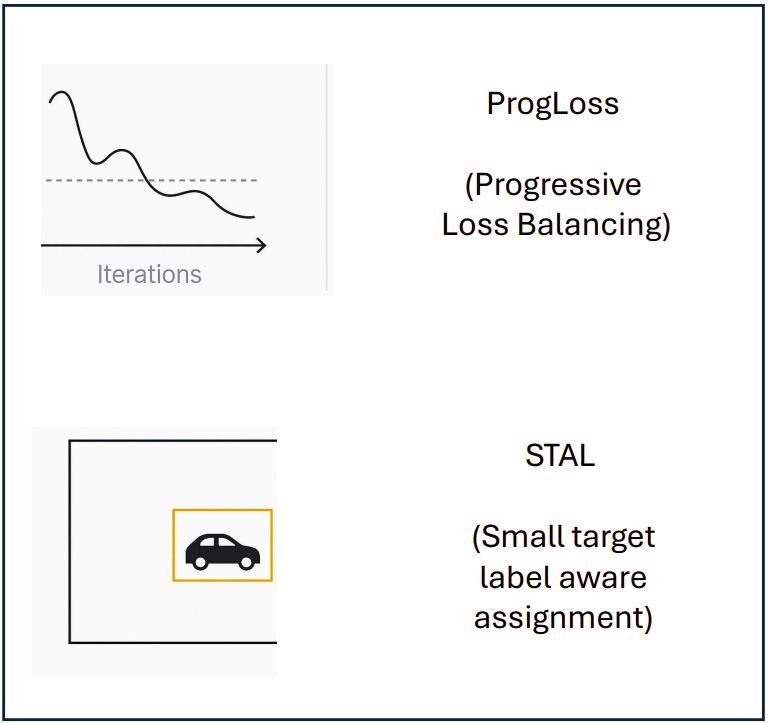
\includegraphics[height=5cm, keepaspectratio]{Figures/Chapter2/Chapter2_6.png}
    \caption{Tối ưu cho vật thể nhỏ~\cite{Reference18}}
    \label{fig:handwriting_challenges}
\end{figure}


\subsubsection*{4. Trình tối ưu hóa MuSGD}

YOLO26 sử dụng trình tối ưu hóa MuSGD, kết hợp giữa Stochastic Gradient Descent (SGD) và thuật toán Muon. Phương pháp này giúp cải thiện tốc độ hội tụ và đảm bảo sự ổn định trong quá trình huấn luyện\cite{Reference18}.

Việc áp dụng MuSGD cho phép mô hình đạt hiệu năng cao mà vẫn duy trì độ ổn định khi huấn luyện trên các tập dữ liệu lớn.

\begin{figure}[H]
    \centering
    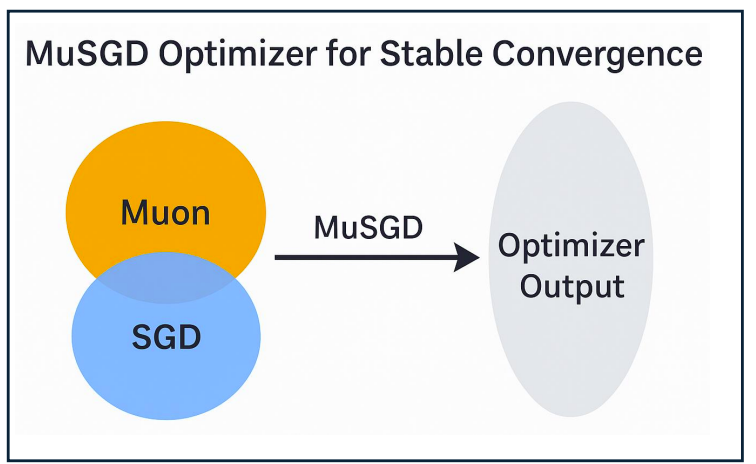
\includegraphics[height=5cm, keepaspectratio]{Figures/Chapter2/Chapter2_7.png}
    \caption{Tối ưu hóa MuSGD~\cite{Reference18}}
    \label{fig:handwriting_challenges}
\end{figure}

Nhờ đó, YOLO26 có thể được sử dụng như một nền tảng thống nhất cho nhiều ứng dụng khác nhau trong thị giác máy tính.

\section{Mạng CRNN}

Tên đầy đủ của CRNN là \textit{Convolutional Recurrent Neural Network}, là một kiến trúc mạng nơ-ron kết hợp những ưu điểm của mạng nơ-ron tích chập (CNN) và mạng nơ-ron hồi quy (RNN) \cite{Reference5,Reference16,Reference17}.

\begin{figure}[H]
    \centering
    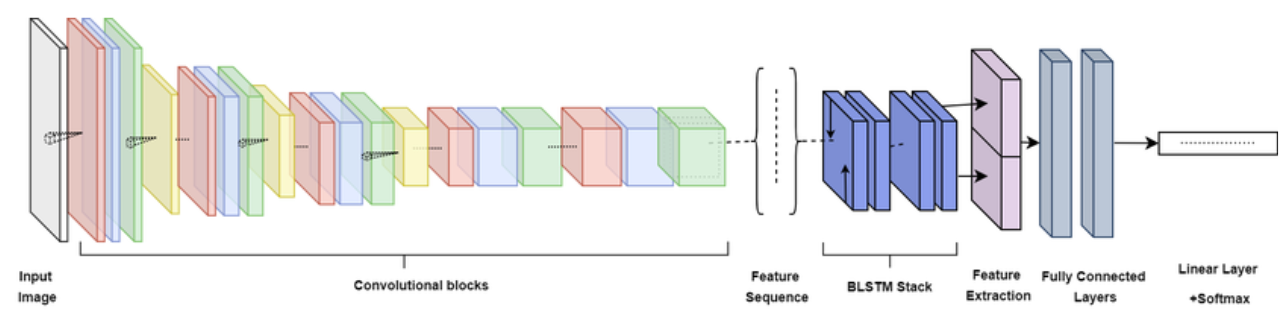
\includegraphics[width=0.9\linewidth]{Figures/Chapter3/Chapter3_6.png}
    \caption{Mạng CRNN tổng quát~\cite{Reference5}}
    \label{fig:handwriting_challenges}
\end{figure}

Mạng nơ-ron hồi quy tích chập (CRNN) thường được sử dụng để xử lý và phân loại dữ liệu chuỗi như giọng nói, văn bản và hình ảnh. Khả năng xử lý dữ liệu chuỗi có độ dài thay đổi và nắm bắt các mối quan hệ phụ thuộc dài hạn khiến mô hình đặc biệt hiệu quả trong các nhiệm vụ yêu cầu hiểu và mô hình hóa thông tin ngữ cảnh và thời gian. CRNN là một công cụ mạnh mẽ để mô hình hóa và xử lý dữ liệu chuỗi, thể hiện hiệu suất tốt trong nhiều bài toán khác nhau \cite{Reference5}.

% \begin{figure}[H]
%     \centering
%     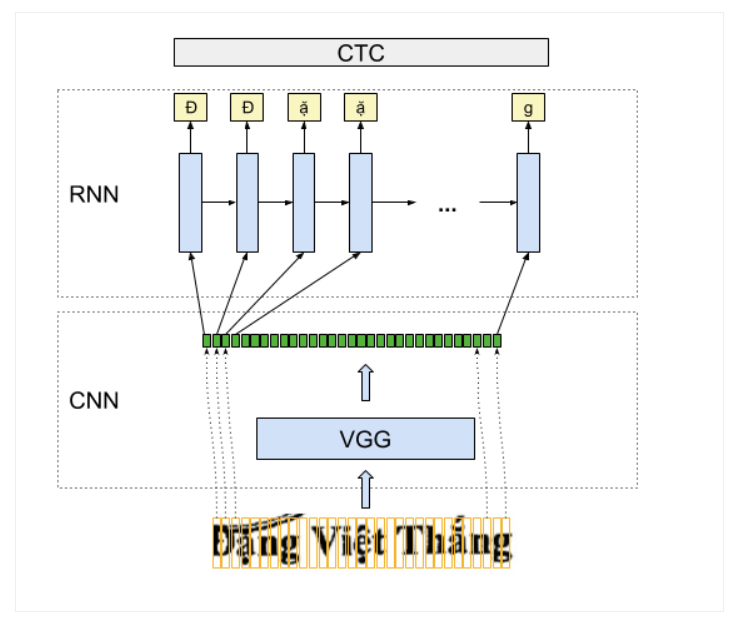
\includegraphics[height=10cm, keepaspectratio]{Figures/Chapter2/Chapter2_8.png}
%     \caption{Kiến trúc mô hình}
%     \label{fig:handwriting_challenges}
% \end{figure}
\subsection{Mạng CNN}

Kiến trúc mạng nơ-ron tích chập (CNN) trong sơ đồ được xây dựng theo mô hình học sâu điển hình, bao gồm hai thành phần chính là khối trích xuất đặc trưng (\textit{Feature Extraction}) và khối phân loại/quyết định (\textit{Classification}) \cite{Reference16}. 

Hệ thống tiếp nhận ảnh đầu vào dưới dạng dữ liệu thô, sau đó xử lý tuần tự qua nhiều tầng trung gian nhằm tự động học và trích xuất các đặc trưng quan trọng của ảnh. Những đặc trưng này tiếp tục được đưa vào khối phân loại để thực hiện quá trình dự đoán và tính toán giá trị chi phí ở đầu ra, từ đó hỗ trợ mô hình tối ưu hóa độ chính xác trong quá trình huấn luyện.

\begin{figure}[H]
    \centering
    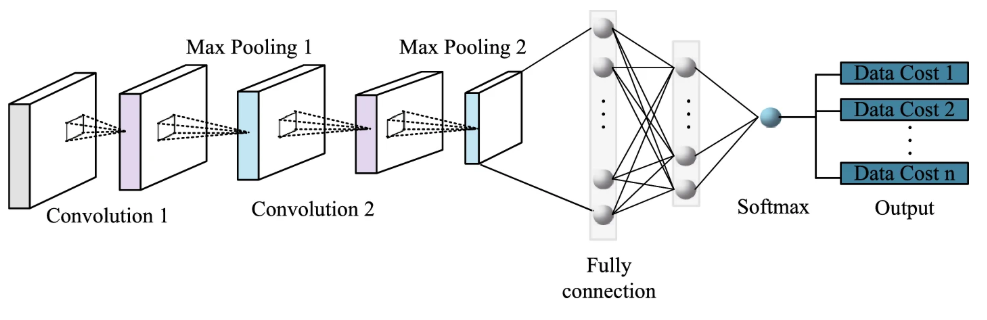
\includegraphics[width=0.9\linewidth]{Figures/Chapter2/Chapter2_10.png}
    \caption{Kiến trúc mạng CNN~\cite{Reference16}}
    \label{fig:cnn_architecture}
\end{figure}

\subsection*{1. Khối trích xuất đặc trưng}

Đây là giai đoạn quan trọng nhất giúp mạng học và hiểu được nội dung của hình ảnh thông qua quá trình lọc và thu gọn thông tin.

\textbf{1. Lớp tích chập}

Các lớp tích chập sử dụng tập hợp các bộ lọc (\textit{kernels}) có kích thước nhỏ di chuyển trên toàn bộ bề mặt ảnh đầu vào. Tại mỗi vị trí, phép tích chập giữa bộ lọc và vùng ảnh cục bộ được thực hiện nhằm tạo ra các bản đồ đặc trưng (\textit{feature maps}).

Lớp Convolution đầu tiên thường có nhiệm vụ phát hiện các đặc trưng hình học cơ bản như cạnh, đường thẳng hoặc điểm ảnh nổi bật. Các lớp Convolution phía sau tiếp tục kết hợp những đặc trưng đơn giản này để hình thành các đặc trưng phức tạp hơn như hình dạng, họa tiết hoặc cấu trúc bề mặt.

\textbf{2. Lớp gộp cực đại}

Được bố trí xen kẽ sau các lớp tích chập, lớp Max Pooling thực hiện việc chọn giá trị lớn nhất trong một cửa sổ trượt (ví dụ: $2 \times 2$) để đại diện cho vùng dữ liệu tương ứng.

Quá trình này giúp giảm kích thước không gian của dữ liệu, từ đó giảm số lượng tham số cần huấn luyện và hạn chế hiện tượng quá khớp (\textit{overfitting}). Đồng thời, Max Pooling còn giúp mô hình đạt được tính bất biến không gian (\textit{spatial invariance}), cho phép mạng vẫn nhận diện được đặc trưng ngay cả khi đối tượng bị dịch chuyển nhẹ trong ảnh.

\subsection*{2. Khối kết nối đầy đủ và phân loại}

Sau khi các đặc trưng quan trọng đã được trích xuất và thu gọn, dữ liệu sẽ được đưa vào khối phân loại để thực hiện quá trình suy luận và ra quyết định.

\textbf{1. Lớp kết nối đầy đủ}

Tại đây, các bản đồ đặc trưng nhiều chiều sẽ được trải phẳng (\textit{flatten}) thành một vector một chiều. Mỗi neuron trong lớp Fully Connected sẽ kết nối với toàn bộ neuron của lớp trước đó. Vai trò của lớp này là thực hiện các phép kết hợp phi tuyến giữa các đặc trưng đã học nhằm đưa ra suy luận cuối cùng về dữ liệu đầu vào.

\textbf{2. Hàm Softmax}

Softmax là hàm kích hoạt cuối cùng của mạng trước khi xuất ra kết quả dự đoán. Hàm này chuẩn hóa các giá trị đầu ra (\textit{logits}) thành phân phối xác suất.

Mỗi giá trị đầu ra sẽ nằm trong khoảng $[0,1]$ và tổng tất cả các xác suất bằng $1$. Điều này cho phép mô hình biểu diễn mức độ tin cậy đối với từng lớp hoặc từng giả thuyết tương ứng.

\subsection*{3.Cấu trúc đầu ra}

Khác với các mạng phân loại ảnh truyền thống thường trả về nhãn đối tượng, đầu ra của kiến trúc này được biểu diễn dưới dạng tập hợp các giá trị \textit{Data Cost} từ $1$ đến $n$.

Trong các bài toán xử lý tín hiệu và thị giác máy tính, \textit{Data Cost} biểu thị mức độ sai số hoặc chi phí phạt khi gán một nhãn hay trạng thái cụ thể cho dữ liệu đầu vào. Mục tiêu của quá trình huấn luyện là cực tiểu hóa các giá trị chi phí này nhằm đạt được kết quả tối ưu.

Việc mô hình xuất ra nhiều giá trị \textit{Data Cost} cho thấy mạng đang đánh giá đồng thời nhiều giả thuyết hoặc nhiều mức độ sai lệch khác nhau. Hệ thống sau đó sẽ lựa chọn kết quả có chi phí nhỏ nhất, tương ứng với phương án có độ chính xác cao nhất.

\subsection{Mạng RNN}

Mạng nơ-ron hồi quy (RNN - Recurrent Neural Network) là một lớp (class) của mạng nơ-ron nhân tạo được thiết kế đặc biệt để xử lý dữ liệu có tính tuần tự (sequential data) hoặc dữ liệu chuỗi thời gian (time-series). Các ứng dụng phổ biến bao gồm xử lý ngôn ngữ tự nhiên (dịch máy, sinh văn bản), nhận dạng giọng nói, và dự báo chuỗi thời gian \cite{Reference5}.

Điểm khác biệt lớn nhất giữa RNN và mạng nơ-ron truyền thẳng truyền thống (Feedforward Neural Network) là RNN sở hữu "trí nhớ". Trong khi mạng truyền thẳng xử lý các đầu vào một cách độc lập, RNN có khả năng lưu giữ thông tin từ các bước tính toán trước đó để gây ảnh hưởng đến kết quả của bước hiện tại. Điều này được thực hiện thông qua các kết nối hồi quy tạo thành một vòng lặp có hướng trong kiến trúc mạng.

\begin{figure}[H]
    \centering
    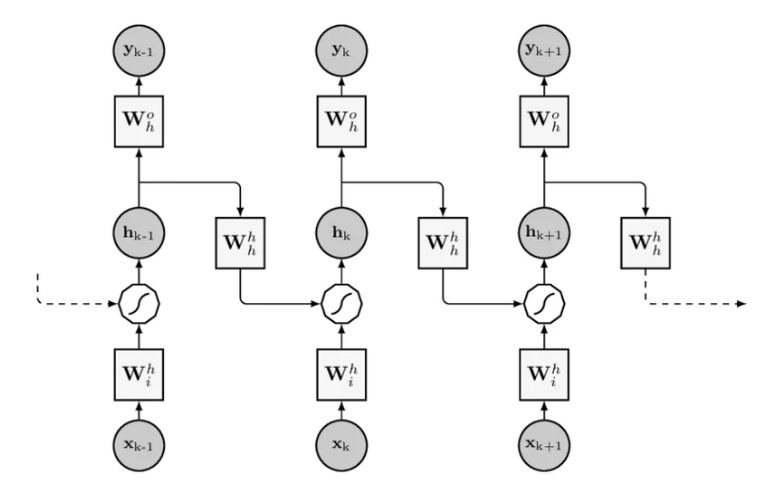
\includegraphics[width=0.9\linewidth]{Figures/Chapter2/Chapter2_11.png}
    \caption{Kiến trúc mạng RNN~\cite{Reference5}}
    \label{fig:rnn_architecture}
\end{figure}

Hình \ref{fig:rnn_architecture} mô tả cấu trúc của một mạng RNN được "trải ra theo thời gian" (unrolled through time). Việc trải mạng giúp minh họa rõ quá trình luồng dữ liệu đi qua mạng tại từng bước thời gian riêng biệt (ví dụ: $k-1$, $k$, và $k+1$).

\subsubsection*{Các thành phần và ký hiệu}
\begin{itemize}
    \item $\mathbf{x}_k$: Véc-tơ dữ liệu đầu vào tại bước thời gian $k$.
    \item $\mathbf{h}_k$: Trạng thái ẩn (hidden state) tại bước $k$. Thành phần này đóng vai trò là "bộ nhớ" của mạng, lưu giữ thông tin tóm tắt về chuỗi dữ liệu tính đến thời điểm hiện tại.
    \item $\mathbf{y}_k$: Véc-tơ đầu ra (output) tại bước $k$.
    \item Các ma trận trọng số (Weight Matrices) cần học trong quá trình huấn luyện:
    \begin{itemize}
        \item $\mathbf{W}_i^h$: Trọng số kết nối từ lớp đầu vào đến trạng thái ẩn.
        \item $\mathbf{W}_h^h$: Trọng số kết nối từ trạng thái ẩn của bước trước đến trạng thái ẩn của bước hiện tại. Đây là ma trận cốt lõi tạo nên vòng lặp hồi quy.
        \item $\mathbf{W}_h^o$: Trọng số kết nối từ trạng thái ẩn đến lớp đầu ra.
    \end{itemize}
\end{itemize}

\subsubsection*{Nguyên lý hoạt động tại một bước thời gian $k$}
Quá trình xử lý thông tin tại bước thời gian $k$ diễn ra theo các bước sau:

\textbf{1. Cập nhật trạng thái ẩn} \\
Để tính toán trạng thái ẩn mới $\mathbf{h}_k$, mạng kết hợp dữ liệu đầu vào hiện tại $\mathbf{x}_k$ và trạng thái ẩn từ bước ngay trước đó $\mathbf{h}_{k-1}$. Tổng tuyến tính của chúng được cộng thêm một véc-tơ độ lệch (bias) $\mathbf{b}_h$ và đưa qua một hàm kích hoạt phi tuyến $f$ (thường là $\tanh$ hoặc $\text{ReLU}$):
$$ \mathbf{h}_k = f(\mathbf{W}_i^h \mathbf{x}_k + \mathbf{W}_h^h \mathbf{h}_{k-1} + \mathbf{b}_h) $$

\textbf{2. Tính toán đầu ra} \\
Sau khi trạng thái ẩn hiện tại $\mathbf{h}_k$ được tính toán, nó được sử dụng để sinh ra đầu ra $\mathbf{y}_k$ tương ứng. Quá trình này thực hiện bằng cách nhân $\mathbf{h}_k$ với ma trận $\mathbf{W}_h^o$, cộng thêm độ lệch $\mathbf{b}_o$ và đưa qua hàm kích hoạt đầu ra $g$ (ví dụ như Softmax cho các bài toán phân loại):
$$ \mathbf{y}_k = g(\mathbf{W}_h^o \mathbf{h}_k + \mathbf{b}_o) $$

\textbf{3. Truyền trạng thái và chia sẻ trọng số} \\
Trạng thái ẩn $\mathbf{h}_k$ vừa tạo ra không chỉ dùng để tính $\mathbf{y}_k$ mà sẽ tiếp tục được truyền sang bước thời gian $k+1$. Một đặc tính đặc biệt quan trọng có thể quan sát trên Hình \ref{fig:cnn_architecture} là các ma trận trọng số ($\mathbf{W}_i^h$, $\mathbf{W}_h^h$, $\mathbf{W}_h^o$) được sử dụng lặp lại giống hệt nhau ở mọi bước thời gian. Việc chia sẻ trọng số này giúp giảm thiểu đáng kể số lượng tham số cần tối ưu hóa và cho phép mô hình linh hoạt xử lý các chuỗi đầu vào có độ dài bất kỳ.


\subsection{Mạng BiLSTM}

Mặc dù RNN hay các biến thể như LSTM truyền thống đã giải quyết tốt việc ghi nhớ thông tin từ quá khứ, chúng vẫn tồn tại một hạn chế cốt lõi: dữ liệu chỉ được xử lý theo một chiều duy nhất (từ quá khứ đến hiện tại). Tuy nhiên, trong nhiều bài toán thực tế như xử lý ngôn ngữ tự nhiên hay dịch máy, ngữ cảnh từ "tương lai" (các từ xuất hiện phía sau) đóng vai trò quan trọng không kém để hiểu trọn vẹn ý nghĩa của phần tử ở thời điểm hiện tại. Mạng bộ nhớ dài-ngắn hạn hai chiều (BiLSTM - Bidirectional LSTM) được đề xuất nhằm khắc phục triệt để nhược điểm này.

\begin{figure}[H]
    \centering
    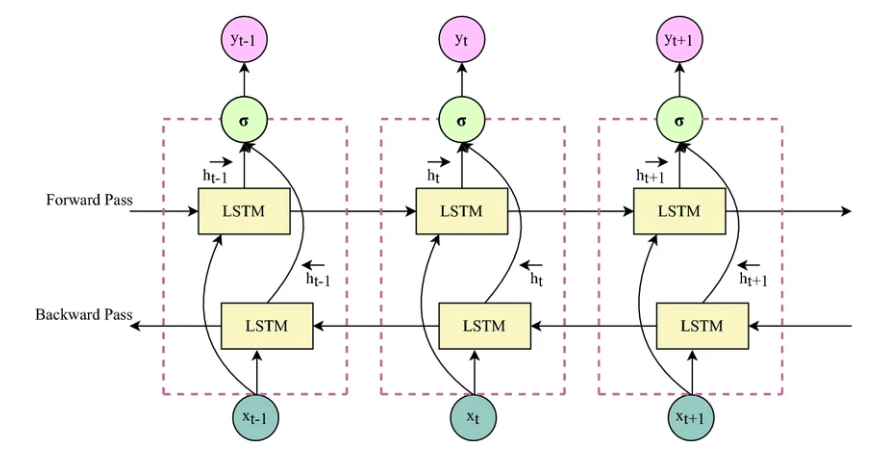
\includegraphics[width=0.9\linewidth]{Figures/Chapter2/Chapter2_12.png} % Thay đổi đường dẫn ảnh cho phù hợp
    \caption{Kiến trúc mạng BiLSTM được trải ra theo thời gian}
    \label{fig:bilstm_architecture}
\end{figure}

Hình \ref{fig:bilstm_architecture} mô tả chi tiết kiến trúc của một mạng BiLSTM được trải ra qua các bước thời gian (ví dụ: $t-1$, $t$, và $t+1$). Thay vì chỉ có một chuỗi ẩn, BiLSTM duy trì hai luồng trạng thái ẩn song song:

\subsubsection*{1. Các thành phần và nguyên lý hoạt động}
\begin{itemize}
    \item \textbf{Lớp truyền xuôi (Forward Pass):} Chuỗi LSTM phía trên (theo chiều mũi tên từ trái sang phải) đọc chuỗi dữ liệu đầu vào $\mathbf{x}$ theo thứ tự thời gian chuẩn (từ $t=1$ đến $T$). Tại bước thời gian $t$, nó tính toán trạng thái ẩn xuôi $\overrightarrow{\mathbf{h}}_t$ dựa trên đầu vào hiện tại $\mathbf{x}_t$ và trạng thái ẩn của bước trước đó $\overrightarrow{\mathbf{h}}_{t-1}$:
    $$ \overrightarrow{\mathbf{h}}_t = \text{LSTM}_{forward}(\mathbf{x}_t, \overrightarrow{\mathbf{h}}_{t-1}) $$

    \item \textbf{Lớp truyền ngược (Backward Pass):} Chuỗi LSTM phía dưới (theo chiều mũi tên từ phải sang trái) đọc chuỗi dữ liệu đầu vào $\mathbf{x}$ theo thứ tự thời gian đảo ngược (từ $t=T$ về $1$). Tại bước thời gian $t$, nó tính toán trạng thái ẩn ngược $\overleftarrow{\mathbf{h}}_t$ dựa trên đầu vào hiện tại $\mathbf{x}_t$ và trạng thái ẩn từ "tương lai" $\overleftarrow{\mathbf{h}}_{t+1}$:
    $$ \overleftarrow{\mathbf{h}}_t = \text{LSTM}_{backward}(\mathbf{x}_t, \overleftarrow{\mathbf{h}}_{t+1}) $$
\end{itemize}

\textbf{2. Tích hợp thông tin và tính toán đầu ra} \\
Tại mỗi bước thời gian $t$, đầu ra cuối cùng của mạng không chỉ phụ thuộc vào quá khứ mà còn dựa vào tương lai. Trạng thái ẩn xuôi $\overrightarrow{\mathbf{h}}_t$ và trạng thái ẩn ngược $\overleftarrow{\mathbf{h}}_t$ được kết hợp lại với nhau (thường là phép nối ghép véc-tơ - concatenation). 

Trong Hình \ref{fig:bilstm_architecture}, sự kết hợp này được biểu diễn bằng các mũi tên từ hai khối LSTM cùng hướng về một nút kích hoạt $\sigma$ (Sigmoid hoặc Softmax tùy bài toán) để tạo ra dự đoán đầu ra $\mathbf{y}_t$:
$$ \mathbf{y}_t = \sigma(\mathbf{W}_y [\overrightarrow{\mathbf{h}}_t \oplus \overleftarrow{\mathbf{h}}_t] + \mathbf{b}_y) $$
Trong đó:
\begin{itemize}
    \item $\oplus$ đại diện cho phép toán nối (concatenate) hoặc cộng hai véc-tơ trạng thái ẩn.
    \item $\mathbf{W}_y$ và $\mathbf{b}_y$ lần lượt là ma trận trọng số và độ lệch của lớp đầu ra.
\end{itemize}

Nhờ kiến trúc song song này, tại bất kỳ thời điểm $t$ nào, mạng BiLSTM đều sở hữu lượng thông tin đầy đủ nhất về toàn bộ chuỗi dữ liệu (cả trước và sau $\mathbf{x}_t$), từ đó đưa ra các dự đoán chính xác và mang tính ngữ cảnh toàn cục cao hơn so với LSTM đơn hướng.